\documentclass[11pt,a4paper]{article}
\usepackage[margin=25mm]{geometry}
\usepackage[T1]{fontenc}
\usepackage{lmodern,amsmath,amssymb,amsthm,mathtools,booktabs,graphicx,microtype,enumitem,xcolor,array}
\usepackage[hidelinks]{hyperref}
\definecolor{ink}{HTML}{4B2840}
\usepackage{titlesec}
\titleformat{\section}{\large\bfseries\color{ink}}{\thesection}{.55em}{}
\titleformat{\subsection}{\normalsize\bfseries}{\thesubsection}{.55em}{}
\newtheorem{theorem}{Theorem}
\newtheorem{lemma}[theorem]{Lemma}
\newtheorem{corollary}[theorem]{Corollary}
\theoremstyle{remark}
\newtheorem{remark}[theorem]{Remark}
\newcommand{\Tr}{\operatorname{Tr}}
\newcommand{\E}{\mathbb E}
\newcommand{\Prob}{\mathbb P}
\newcommand{\dd}{\mathrm d}
\setlength{\parindent}{1em}
\setlength{\emergencystretch}{2em}
\allowdisplaybreaks
\title{\bfseries\color{ink} The energy an isolated half of a critical chain cannot give up\\[3pt]\large Conformal amplitudes, dispersion, and the cost of conserving particle number}
\author{Anonymous\\[3pt]{\small DOI \href{https://doi.org/10.5281/zenodo.24553557}{10.5281/zenodo.24553557}}}
\date{Evidence Press research manuscript}
\begin{document}
\maketitle
\begin{abstract}
Cut a critical quantum chain in two and isolate one half. The half is left in a mixed state, so unitary operations on it can extract work, but some energy above its ground state always remains. Mula and colleagues (2023) called this remainder the bound energy and proposed that it scales as the square of the entanglement entropy divided by the chain length, with a coefficient they computed for the free-fermion chain. We prove this law, with coefficient $3vS^2/(2\pi cL)$, for a regulated boundary conformal field theory, and directly for the open hopping and critical Ising lattice chains; at equal velocity the Ising slope is twice the hopping slope, so the slope depends on the ratio of velocity to central charge and the conjectured number is not universal. For a broad family of free-fermion chains that all share the hopping chain's ground state, we determine the bound energy exactly to leading order: it is fixed by the flattest zero of the one-particle dispersion, and the conjectured form holds if and only if that dispersion has a nonzero velocity at the Fermi level and no other zero. A ground state's criticality therefore does not determine its bound energy. Finally, one range-three chain shows that restricting the allowed operations changes the leading power: unrestricted, particle-number-conserving and one-body number-conserving operations leave residuals of orders $(\log L)^3/L^2$, $(\log L)/L$ and $(\log L)^2/L$. The lattice proofs rest on one external input, the known boundary R\'enyi asymptotics of the open hopping chain. All coefficients are limits as the block length $L$ grows; exact finite-size computations up to $L=4096$ show which of the separations are already visible and which converge only logarithmically slowly.
\end{abstract}

\section{Introduction}\label{sec:intro}
This section explains the question, why it is asked, what was known, what this paper adds, and how the paper is organised.

\paragraph{The problem.} A quantum system in a mixed state $\rho$ with Hamiltonian $H$ generally stores energy that a unitary operation can extract as work. The maximum, the \emph{ergotropy} \cite{allahverdyan}, is reached by rotating $\rho$ into the \emph{passive} state, whose most probable eigenvector is the ground state of $H$, whose second most probable is the first excited state, and so on. A passive state need not be the ground state: if $\rho$ is mixed, some energy is left over. Mula et al.\ \cite{mula} applied this to the ground state of a critical chain. When half of the chain is isolated, its reduced state $\rho_L$ is mixed because of entanglement with the other half. They called the energy that remains above the isolated half's own ground energy after optimal extraction the \emph{bound energy}. We write it $Q_L$ and also call it the residual energy.

\paragraph{Why it matters.} The bound energy links two descriptions of the same block: its entanglement spectrum (the eigenvalues of $\rho_L$) and its physical energy spectrum (the eigenvalues of the block Hamiltonian). It is the work that entanglement makes permanently unavailable to any operation on the block alone. It has been proposed as a thermodynamic probe of criticality \cite{mula,mitra}, and the question of which operations are allowed connects it to work extraction under conservation laws, an active theme in quantum thermodynamics \cite{mitsu,onuma}.

\paragraph{What was known.} For the open free-fermion (XX) chain of $N=2L$ sites, Mula et al.\ derived $NQ_L\approx(6/\pi)S_L^2$, where $S_L$ is the block entanglement entropy \cite[Eq.~(42)]{mula}. Their calculation, Eq.~(34) of \cite{mula}, pairs single-particle occupations with single-particle energies; this is the optimum over one-body rotations, not over all unitaries. Their conjecture appears in three forms, which must be kept apart:
\begin{itemize}[leftmargin=2.2em,itemsep=1pt]
\item[(A)] the abstract of \cite{mula}: the relation holds ``for all 1D critical states'';
\item[(B)] the discussion after their Eq.~(42) and their conclusions: it holds for critical states ``described by a conformal field theory'';
\item[(C)] the formula itself, with the specific slope $6/\pi$.
\end{itemize}
They gave preliminary exact-diagonalisation data for the Ising chain up to $N=14$ and the Heisenberg chain up to $N=24$. Mitra and Srivastava \cite{mitra} studied a long-range Kitaev chain. Their passive energy, like that of Mula et al., is the one-body pairing \cite[Eq.~(22)]{mitra}. At a pairing exponent where conformal symmetry is broken they obtained the same $S^2/N$ law and slope, analytically under an assumed form of the entanglement spectrum, and confirmed it numerically; for nearest-neighbour pairing they reported a fitted slope close to $6/\pi$. For intermediate exponents they found the law numerically with decreasing slopes, they found linear behaviour in exact-diagonalisation data for XY chains, and they saw a clear deviation only for all-to-all pairing. Hartmann, Kavanagh and Vandoren \cite{hartmann} had shown that free fermions with odd Lifshitz dispersion share the ground-state entanglement of ordinary hopping. No proof of any form of the conjecture was available.

\paragraph{What is new.} This paper proves the following.
\begin{enumerate}[leftmargin=2.2em,itemsep=2pt]
\item \emph{A rank-matching principle} (Lemma~\ref{lem:rank}). Asymptotically the bound energy equals the energy of the block Hamiltonian's thermal state whose entropy equals $S_L$. This is the thermodynamic intuition behind every result below; the lemma states hypotheses under which it is exact to leading order.
\item \emph{The conformal law} (Theorems~\ref{thm:cft} and~\ref{thm:boundary}, Corollary~\ref{cor:relative}). In a regulated boundary conformal field theory (CFT), $Q_L\sim3vS_L^2/(2\pi cL)$ for velocity $v$ and central charge $c$, whatever boundary condition the entanglement cut carries. In rational CFTs the next term is fixed by the boundary entropy of the physical termination, and the passive state converges to the strip's thermal state in relative entropy.
\item \emph{Exact lattice laws for one ground state and many Hamiltonians} (Theorem~\ref{thm:general}, Corollaries~\ref{cor:odd}--\ref{cor:ising}). For every sign-preserving polynomial $f$, the chain $\dd\Gamma(f(T))$ has the hopping ground state, and $Q_L\sim D\,S_L^{m+1}/L^m$, where $m$ is the largest order of a zero of the dispersion. The $S^2/L$ form holds if and only if $m=1$. For the hopping and critical Ising chains the slopes are $3/\pi$ and $6/\pi$ in $L$ units, as the CFT predicts.
\item \emph{Stability} (Theorem~\ref{thm:cross}). Adding a linear term to a flat dispersion restores the $S^2/L$ form, through an explicit crossover function.
\item \emph{The cost of restricting the controls} (Theorems~\ref{thm:gauss} and~\ref{thm:three}, Corollaries~\ref{cor:charge} and~\ref{cor:pq}). One-body rotations can leave strictly more energy than unrestricted unitaries, and in a single range-three chain the unrestricted, charge-conserving and charge-conserving one-body classes give three different leading orders in $L$.
\end{enumerate}
For the three forms of the conjecture this means: (A) is false; (B) holds for the regulated CFT spectra and for the hopping and Ising lattice chains, and remains open for interacting lattice chains such as the Heisenberg chain; (C) holds for unit hopping but not in general, since the slope is $3v/(\pi c)$ in units of $N$; the statement free of energy units is $LQ_L/(vS_L^2)\to3/(2\pi c)$. Section~\ref{sec:discussion} collects this in Table~\ref{tab:status}.

\paragraph{What is not claimed.} The lattice proofs concern free-fermion chains. No interacting lattice chain is treated. The allowed unitaries have no limit on depth, locality or duration, so the theorems describe what any operation on the block could achieve, not a protocol. The coefficients are limits as $L\to\infty$; because the entropy grows only like $\tfrac16\log L$, some of them are approached very slowly (Section~\ref{sec:numerics}).

\paragraph{Roadmap.} Section~\ref{sec:setting} fixes notation, defines the control classes and proves the rank-matching lemma. Section~\ref{sec:cft} treats the conformal interval. Section~\ref{sec:lattice} proves the lattice laws for the family sharing one ground state, and Section~\ref{sec:ising} the Ising chain. Section~\ref{sec:crossover} studies the crossover to linear dispersion. Section~\ref{sec:controls} compares control classes. Section~\ref{sec:numerics} reports finite-size computations, and Section~\ref{sec:discussion} summarises the status of the conjecture and open problems. Appendices~\ref{app:renyi}--\ref{app:charge} contain the entanglement asymptotics and the charge-sector counting.

\section{Setting, notation and the rank-matching principle}\label{sec:setting}
This section defines the residual energy and the control classes, collects notation, and proves the lemma that converts entropy and level counting into the residual energy.

Cut an open chain of $N=2L$ sites at its centre. The left block has reduced state $\rho_L$ and, after the terms crossing the cut are deleted, Hamiltonian $H_L$ with ground energy $E_0$. The residual energy is
\begin{equation}
 Q_L=\min_U\Tr(U\rho_L U^\dagger H_L)-E_0=\sum_{r\ge1}p_r\mathcal E_r,\qquad S_L=-\sum_r p_r\log p_r .
 \label{eq:def}
\end{equation}
Here $p_1\ge p_2\ge\cdots$ are the eigenvalues of $\rho_L$, $0=\mathcal E_1\le\mathcal E_2\le\cdots$ are the excitation energies $E_r-E_0$ of $H_L$, both lists count multiplicity, and the minimum is over all unitaries $U$ on the block. The equality is the rearrangement inequality for traces: the largest probabilities go on the cheapest levels \cite{allahverdyan}. The work extracted is $\Tr(\rho_LH_L)-E_0-Q_L$. The site spacing, $\hbar$ and $k_B$ are one, hopping amplitudes are one, and entropies are in nats.

\paragraph{Control classes.} Besides the unrestricted minimum $Q_L$ we consider three restricted ones for fermion chains with block particle number $n$: $Q_L^{\rm ch}$, the minimum over unitaries commuting with $n$ (charge-conserving); $Q_L^{\rm G}$, the minimum over number-conserving fermionic Gaussian unitaries, that is, rotations of the single-particle modes; and $Q_L^{\rm pair}$, the minimum over all fermionic Gaussian unitaries, which may create particles in pairs. Since each class contains the next, $Q_L\le Q_L^{\rm ch}\le Q_L^{\rm G}$ at every $L$. The quantity computed by Mula et al.\ is $Q_L^{\rm G}$.

\begin{table}[htbp]\centering\small
\caption{Notation used throughout.}\label{tab:notation}
\begin{tabular}{>{\raggedright}p{.21\linewidth}p{.71\linewidth}}
\toprule
Symbol & Meaning\\
\midrule
$L$, $N=2L$, $d$ & block length, chain length, $d=\log L$\\
$\rho_L$, $p_r$, $S_L$ & block state, its ordered eigenvalues, its entropy\\
$H_L$, $E_0$, $\mathcal E_r$ & block Hamiltonian after the cut, its ground energy, ordered excitation energies\\
$Q_L$, $Q_L^{\rm ch}$, $Q_L^{\rm G}$, $Q_L^{\rm pair}$ & residual energy under unrestricted, charge-conserving, number-conserving Gaussian and general Gaussian control\\
$R$ & random rank with law $\Prob(R=r)=p_r$\\
$v$, $c$ & velocity and central charge of a CFT\\
$h_e(r)$, $h_p(r)$ & ordered conformal weights (above the lowest) of the entanglement and physical boundary problems\\
$u$, $W$, $K_x$, $G_x$ & entanglement temperature $u=2\pi^2/W$, regulated width $W$, Cardy constant, boundary degeneracy factor\\
$T_M$ & adjacency matrix of the open path on $M$ sites\\
$\dd\Gamma(B)$ & $\sum_{ij}B_{ij}c_i^\dagger c_j$, the many-body operator of a one-body matrix $B$\\
$f$, $m$, $\kappa_a$, $A$, $D(m,A)$ & one-body polynomial, largest zero order, stiffness at a zero $a$, pressure constant, residual coefficient (Theorem~\ref{thm:general})\\
$z$, $A_z$, $D_z$ & odd power in $f(x)=x^z$ and its constants (Corollary~\ref{cor:odd})\\
$\eta(s)$ & Dirichlet eta function $(1-2^{1-s})\zeta(s)$\\
$\nu_j$, $x_j$ & block correlation eigenvalues and single-particle entanglement energies $|\log((1-\nu_j)/\nu_j)|$\\
$a_j$, $w_j^\pm$, $n_*$ & ordered one-body costs; particle ($+$) and hole ($-$) costs; number of negative one-body levels\\
\bottomrule
\end{tabular}
\end{table}

The next lemma is the common engine of all leading-order results. It says that the residual energy is the energy at the rank occupied by a typical Schmidt probability.

\begin{lemma}[Rank matching]\label{lem:rank}
For each $L$ let $p_r$ and $\mathcal E_r$ be as in \eqref{eq:def}, let $u_L\to\infty$ and $g_L>0$, and let $R$ be a random rank with $\Prob(R=r)=p_r$. Suppose that
\begin{enumerate}[label=(\alph*),itemsep=1pt]
\item $\log R/u_L\to1$ in probability, and $\E[(\log(1+R)/u_L)^k]$ is bounded in $L$ for every $k>0$;
\item there is a continuous, strictly increasing $\varphi$ on $(0,\infty)$ with $\mathcal E_{r_L}/g_L\to\varphi(x)$ whenever $\log r_L/u_L\to x>0$;
\item $\mathcal E_r\le Cg_L(1+\log r/u_L)^{\gamma}$ for all $r$ and $L$, with constants $C,\gamma$.
\end{enumerate}
Then $Q_L/g_L\to\varphi(1)$.
\end{lemma}
\begin{proof}
Fix $\delta\in(0,1)$. On the event $|\log R/u_L-1|\le\delta$, monotonicity of $\mathcal E_r$ in $r$ places $\mathcal E_R$ between $\mathcal E_{r_-}$ and $\mathcal E_{r_+}$, where $r_\pm=\lceil e^{(1\pm\delta)u_L}\rceil$. By (b) these are $g_L[\varphi(1\pm\delta)+o(1)]$. Since the event has probability tending to one and $\varphi$ is continuous, $\mathcal E_R/g_L\to\varphi(1)$ in probability. By (c) and (a), $\E[(\mathcal E_R/g_L)^2]$ is bounded, so the family is uniformly integrable and $Q_L/g_L=\E[\mathcal E_R/g_L]\to\varphi(1)$.
\end{proof}

\begin{remark}[Isentropic reading]\label{rem:isentropic}
In every application below, (b) comes from a level count $u_L^{-1}\log\#\{r:\mathcal E_r\le eg_L\}\to\sigma(e)$, and then $\varphi=\sigma^{-1}$. The value $\varphi(1)$ is the energy at which the block Hamiltonian's microcanonical entropy equals $S_L$ to leading order, which is the energy of its thermal state with entropy $S_L$. The lemma is therefore a rigorous version of the isentropic heuristic, familiar from the many-copy analysis of Alicki and Fannes \cite{alicki}, for a single block whose state and Hamiltonian both change with $L$. The work in each theorem lies in verifying (a)--(c), especially the tail bound (c), which controls ranks far beyond the typical one.
\end{remark}

\section{A conformal interval after isolation}\label{sec:cft}
This section proves the conformal form of the law when both the entanglement spectrum and the physical spectrum are given by boundary CFT, and identifies the first correction.

Consider the end interval of a finite open system with the same conformal boundary condition at its two original ends. In the Cardy--Tonni regularisation \cite{tonni,alba}, the reduced state has ordered eigenvalues
\[
 p_r=e^{-u h_e(r)}/Z_e(u),\quad Z_x(t)=\sum_{r\ge1}e^{-t h_x(r)},\quad u=2\pi^2/W .
\]
We choose $h_x(r)=\Delta_x(r)-\Delta_{x,0}\ge0$, the gap in conformal weight; a common shift has no physical effect. For a half of length $L$ and short-distance cutoff $\epsilon$, $W=\log[4L/(\pi\epsilon)]+o(1)$, so $u\to0$. The physical open strip of length $L$ has $\mathcal E_r=(\pi v/L)h_p(r)$ \cite{cardy}. The subscripts $e$ and $p$ label the entanglement and the physical boundary problems, which may carry different boundary conditions. Fixing any identification of their bases gives the same unrestricted minimum in \eqref{eq:def}. This is a model of the reduced state: for a lattice chain, whether the Schmidt spectrum follows it at the large ranks that matter is a separate question, answered below only for free chains.

\begin{theorem}[Conformal amplitude]\label{thm:cft}
Suppose the two spectra are discrete with finite multiplicities, the partition functions converge for every $t>0$, and $\log Z_x(t)\sim K_x/t$ as $t\downarrow0$ with $K_x>0$. Then
\[
 Q_L\sim \frac{\pi v}{4K_p L}S_L^2 .
\]
For annulus and strip sectors of a unitary CFT of central charge $c>0$ whose closed channel is dominated by the vacuum, $K_p=\pi^2 c/6$, and hence
\begin{equation}
 \boxed{\displaystyle Q_L\sim\frac{3v}{2\pi c}\frac{S_L^2}{L}.}
 \label{eq:cft}
\end{equation}
\end{theorem}
\begin{proof}
Write $N_x(H)=\#\{r:h_x(r)\le H\}$. The bound $N_x(H)\le e^{tH}Z_x(t)$, optimised at $t=\sqrt{K_x/H}$, gives $\limsup H^{-1/2}\log N_x(H)\le 2\sqrt{K_x}$. Under the Gibbs weights at $t$, $t^2 h_x\to K_x$ in probability: at speed $1/t$ the scaled log moment generating function converges to $K_x[(1-s)^{-1}-1]$ for $s<1$, and exponential Markov bounds on both sides of zero give concentration at its derivative. The Gibbs probability of the band $(1\pm\delta)K_x/t^2$ therefore tends to one, so the count below $(1+\delta)K_x/t^2$ is at least $Z_x(t)e^{(1-\delta)K_x/t}(1-o(1))$. Letting $\delta\to0$ gives the reverse inequality, and inverting the cumulative count, ties included, gives $h_x(r)\sim(\log r)^2/(4K_x)$.

Write $\E_u$ for expectation under the Gibbs weights $p_r$ at $u$. Convexity of $\log Z_e$ and the difference quotients at $(1\pm\delta)u$ give $\E_u h_e\sim K_e/u^2$, so $S_L=\log Z_e+u\E_u h_e\sim 2K_e/u$. For the random rank, $\log R=2\sqrt{K_eh_e(R)}(1+o(1))$ and $u^2h_e(R)\to K_e$ in probability, so $\log R/S_L\to1$; the exponential tails of $uh_e$ under the Gibbs law give the moment bound in Lemma~\ref{lem:rank}(a). Condition (b) holds with $u_L=S_L$, $g_L=S_L^2/L$ and $\varphi(x)=\pi vx^2/(4K_p)$, by the asymptotic for $h_p$. For (c), the count asymptotic gives $N_p(H)\ge e^{\sqrt{K_pH}}$ for $H\ge H_0$, hence $h_p(r)\le H_0+(\log r)^2/K_p$ for all $r$. Lemma~\ref{lem:rank} gives the result. For the vacuum-dominated annulus, modular exchange gives the stated $K_x$ \cite{cardy,alba}.
\end{proof}
Only $K_p$ enters the coefficient: the entanglement boundary condition affects $S_L$ but not the relation between $Q_L$ and $S_L$. When the two spectra coincide, the passive state is exactly the strip's Gibbs state at inverse temperature $uL/(\pi v)$. The count $h_e(r)\sim(\log r)^2/(4K_e)$ is the CFT distribution of entanglement eigenvalues obtained by Calabrese and Lefevre \cite{calabrese}.

\subsection{The physical boundary fixes the next term}
This subsection identifies the term linear in $S_L$ for rational CFTs. Assume that each open-channel spectrum is a finite nonnegative sum of characters with rational conformal weights, with a finite-dimensional modular transformation, a positive vacuum overlap $G_x$, and a gap above the unique bulk vacuum in the closed channel. In the usual boundary-state convention $G_x=g_{a_x}g_{b_x}$, the product of the boundary entropies of the two ends. Write $K=\pi^2 c/6$.

\begin{theorem}[Boundary correction]\label{thm:boundary}
Under these hypotheses the unrestricted residual energy obeys
\begin{equation}
 \frac{LQ_L}{\pi v}=
 \frac{(S_L-\log G_p)^2}{4K}+o(S_L).
 \label{eq:boundary}
\end{equation}
This identifies the term linear in $S_L$; no claim is made for the constant term.
\end{theorem}
\begin{proof}
The modular transformation gives, as $w\to0$ in each fixed cone $|\Im w|\le M\Re w$,
\[
 Z_x(w)=G_x\exp(K/w+d_x w)
 \{1+O(\exp[-b_x\Re(1/w)])\},\qquad b_x>0 .
\]
The constant $d_x$ records the choice of zero of conformal weight. Each character at the transformed modulus is vacuum dominated in that cone, which also gives $|Z_x(w)|\le C_M e^{K/|w|}$. The cumulative form of Ingham's Tauberian theorem \cite[Theorem 1.1]{ingham} therefore gives
\begin{equation}
 N_x(H)\sim\frac{G_x}{2\sqrt{\pi}(KH)^{1/4}}e^{2\sqrt{KH}} .
 \label{eq:count2}
\end{equation}
For example, on a grid with $m h_x\in\mathbb Z$, apply that theorem to $Z_x(mw)$ at index $\lfloor mH\rfloor$; the product of the exponential constant $K/m$ and the index is asymptotic to $KH$. Equation~\eqref{eq:count2} implies $N_x(H-1/m)/N_x(H)\to1$, so every rank in a degenerate level has $\log r=\log N_x(h_x(r))+o(1)$.

At a common rank the proof of Theorem~\ref{thm:cft} gives $h_p/h_e\to1$. Equating the logarithms in \eqref{eq:count2} cancels the logarithmic terms up to $o(1)$ and gives
\[
 h_p-h_e=\log(G_e/G_p)\sqrt{h_e/K}+o(\sqrt{h_e}).
\]
The Gibbs law has $u^2 h_e\to K$ in probability, and the bounded second moment of $u^2h_e$ makes $u\sqrt{h_e}$ uniformly integrable, so $\E_u\sqrt{h_e}\sim\sqrt K/u$. On the real axis the modular expansion holds uniformly on discs of radius proportional to $u$ about $u$ inside a cone, so Cauchy's estimate allows it to be differentiated: $\E_u h_e=-\partial_u\log Z_e=K/u^2+O(1)$ and $S_L=2K/u+\log G_e+o(1)$. Averaging the rank difference, with finitely many low levels contributing $O(1)$, gives $LQ_L/(\pi v)=K/u^2+\log(G_e/G_p)/u+o(1/u)$. Substitution yields \eqref{eq:boundary}.
\end{proof}
\begin{corollary}[Thermal form of the passive state]\label{cor:relative}
In Theorem~\ref{thm:boundary}, let $P_u$ be the passive (reordered) state and $T_u$ the physical strip's Gibbs state at dimensionless inverse temperature $u$, that is, physical inverse temperature $uL/(\pi v)$. Then $D(P_u\Vert T_u)\to0$, $D(T_u\Vert P_u)\to0$, and $\|P_u-T_u\|_1\to0$.
\end{corollary}
\begin{proof}
In a common rank basis, $D(P_u\Vert T_u)=u\E_e h_p+\log Z_p(u)-S_L$. The preceding proof gives $u\E_e h_p=K/u+\log(G_e/G_p)+o(1)$, and $\log Z_p(u)=K/u+\log G_p+o(1)$. Substitution cancels both the diverging term and the constant. Exchanging the two spectra gives the reverse divergence, because the rank ordering is the same. Pinsker's inequality gives the trace-norm limit.
\end{proof}
Corollary~\ref{cor:relative} answers, for these spectra, the question raised at the end of \cite{mula} about the properties of the passive state under the block's own Hamiltonian: it is asymptotically thermal for that Hamiltonian, at a physical temperature $\pi v/(uL)$ that tends to zero. The cut itself supplies no relaxation dynamics; the statement concerns the optimally rearranged state.

\paragraph{A continuum illustration.} For the Ising CFT, take the entanglement cut and the outer end free and terminate the isolated strip with a fixed spin. Then $G_e=g_{\rm free}^2=1$ and $G_p=g_{\rm free}g_{\rm fixed}=1/\sqrt2$ \cite{cardy}, and the correction replaces $S_L$ by $S_L+\tfrac12\log 2$ at this precision. Table~\ref{tab:checks} checks this inside the continuum model. It is an illustration of Theorem~\ref{thm:boundary}, not a lattice prediction: the free entanglement condition is an assumption, the unaltered lattice cut has free ends with $G_p=1$, and a fixed termination would have to be added by the experimenter. For the unaltered lattice Ising cut, $G_p=G_e=1$ and the predicted linear shift vanishes; the lattice offset $2\sqrt{K LQ_L/(\pi v)}-S_L$ falls slowly, from $0.056$ at $L=16$ to $0.038$ at $L=2048$. A proof of the linear term on the lattice is not attempted here.

\section{One ground state, many residual energies}\label{sec:lattice}
This section proves the residual-energy law directly on the lattice for a family of free-fermion chains that all share one ground state, and shows exactly when the conformal form holds within this family.

Let $T_M$ be the adjacency matrix of the open path of $M$ sites. For a real polynomial $f$ of degree $D$ consider the chain $H_{2L}=\dd\Gamma(f(T_{2L}))$, a fermion hopping Hamiltonian of range $D$; the Jordan--Wigner map turns it into a finite-range spin chain. The eigenvalues of $T_M$ are $2\cos k$ with $k=\pi j/(M+1)$, so the bulk one-particle dispersion is $f(2\cos k)$, and the Fermi points of the half-filled chain sit at $k=\pi/2$, where $2\cos k=0$. We call $f$ \emph{sign-preserving} if
\begin{enumerate}[label=(S\arabic*),itemsep=1pt]
\item $xf(x)\ge0$ on $[-2,2]$, $f(0)=0$, $f(\pm2)\ne0$, and $f$ is not identically zero;
\item no eigenvalue of $T_{2L}$ is a zero of $f$.
\end{enumerate}
Condition (S2) holds for every $L$ if each nonzero zero of $f$ in $(-2,2)$ is rational and different from $\pm1$, because the eigenvalues $2\cos(\pi j/(2L+1))$ are algebraic integers and the only rational values of $2\cos(q\pi)$ with $q$ rational are $0,\pm1,\pm2$. Under (S1) the zero at $0$ has odd order $m_0$, and every other zero $a\in(-2,2)$ has even order $m_a$. Let $m$ be the largest of these orders. Near a zero $a$ of order $m_a$ write $f(x)=c_a(x-a)^{m_a}(1+O(x-a))$ and define the stiffness
\[
 \kappa_a=|c_a|\,(4-a^2)^{m_a/2},
\]
so that $|f(2\cos k)|=\kappa_a|k-k_a|^{m_a}(1+O(k-k_a))$ near $k_a=\arccos(a/2)$. Put
\begin{equation}
 A=\frac{2\,\Gamma(1+1/m)\,\eta(1+1/m)}{\pi}\sum_{a:\,m_a=m}\kappa_a^{-1/m},\qquad
 D(m,A)=\frac{m^m}{(m+1)^{m+1}A^m}.
 \label{eq:Aconst}
\end{equation}
The isolated block has the principal compression $B_L=Pf(T_{2L})P$ as its one-body matrix, where $P$ projects on the first $L$ sites; terms crossing the cut are removed.

\begin{theorem}[Residual energy for sign-preserving dispersions]\label{thm:general}
Let $f$ be sign-preserving. Then every chain $\dd\Gamma(f(T_{2L}))$ has the same unique ground state, the half-filled Fermi sea of $T_{2L}$; its block entropy is $S_L=\tfrac16\log L+O(1)$; and
\begin{equation}
 Q_L\sim D(m,A)\,\frac{S_L^{m+1}}{L^m}.
 \label{eq:general}
\end{equation}
\end{theorem}
\begin{proof}
\emph{Ground state.} $T_{2L}$ has no zero eigenvalue because $2L$ is even. For each eigenvalue $\lambda$, (S1) and (S2) give $\lambda f(\lambda)>0$, so $f(T_{2L})$ and $T_{2L}$ have the same negative eigenspace, whose filling is the unique ground state. The reduced state, and in particular $S_L$ and every Schmidt probability, is therefore independent of $f$.

\emph{Schmidt ranks.} Write $I=-\log p_R$. Appendix~\ref{app:renyi} gives, for fixed $q>0$ near one,
\[
 (\log L)^{-1}\log\Tr\rho_L^q\longrightarrow (q^{-1}-q)/12 .
\]
Since $\E e^{tI}=\Tr\rho_L^{1-t}$, exponential Markov bounds on either side of $t=0$ give $I/\log L\to1/6$ with tails exponentially small in $\log L$ outside any fixed neighbourhood. Ranking gives $\log R\le I$. For $d=\log L$, $s=1/6$ and $0<\delta<s$, at most $e^{(s-\delta)d}$ ranks each have probability at most $e^{-(s-\delta/2)d}$ on the event $I\ge(s-\delta/2)d$, so
\[
 \Prob(R\le e^{(s-\delta)d})\le \Prob(I<(s-\delta/2)d)+e^{-\delta d/2}.
\]
Hence $\log R/S_L\to1$ in probability. For fixed small $t>0$, $\E e^{tI}\le e^{C_t d}$, so $\Prob(\log R/d>y)\le e^{-tdy/2}$ for $y>2C_t/t$; every fixed power of $\log(1+R)/S_L$ is uniformly integrable. This is Lemma~\ref{lem:rank}(a) with $u_L=S_L$.

\emph{Physical levels.} The excitation energies of the block are the sorted subset sums of the $L$ one-body costs $|\varepsilon_j(B_L)|$, counting both particles above and holes below zero, so
\[
 \log Z_L(\beta)=\sum_{j=1}^L\log(1+e^{-\beta|\varepsilon_j(B_L)|}).
\]
A path of length $k\le D$ between two block sites that leaves the block must visit site $L+1$, so both endpoints lie among the last $k-1$ block sites. Hence $B_L-f(T_L)$ is supported on the last $D-1$ sites and has rank at most $D-1$. Interlacing bounds the difference of the two eigenvalue counts on any interval $[-h,h]$ by $2(D-1)$, and integrating against the monotone function $\log(1+e^{-\beta h})$ bounds the difference of log partition functions by $2(D-1)\log2$, for all $\beta>0$.

\emph{Pressure.} Put $u_L=S_L$, $g_L=u_L^{m+1}/L^m$ and $\beta=bu_L/g_L=b(L/u_L)^m$. We show that for each $b>0$
\begin{equation}
 \frac{1}{u_L}\log Z_L(\beta)\to F(b)=A\,b^{-1/m}.
 \label{eq:pressure}
\end{equation}
The eigenvalues of $f(T_L)$ are $f(2\cos k_j)$ with $k_j=\pi j/(L+1)$. Fix $\delta>0$ small and surround each zero $k_a$ by the window $|k-k_a|<\delta$. Outside the windows $|f(2\cos k)|\ge c_\delta>0$, so those modes contribute at most $Le^{-\beta c_\delta}\to0$. Inside a window, $|f(2\cos k)|$ lies between $\kappa_a(1\mp C\delta)|k-k_a|^{m_a}$ and is monotone in $|k-k_a|$ on each side, so the sum over the window equals $\frac{L+1}{\pi}\int_{|q|<\delta}\log(1+e^{-\beta|f|})\,\dd q+O(1)$. Scaling $q=(\beta\kappa_a)^{-1/m_a}t$ and using $\int_0^\infty\log(1+e^{-t^{m}})\dd t=\Gamma(1+1/m)\eta(1+1/m)$ shows that a zero of order $m_a$ contributes
\[
 \frac{2(L+1)}{\pi}(\beta\kappa_a)^{-1/m_a}\Gamma(1+1/m_a)\eta(1+1/m_a)(1+O(\delta))+O(1).
\]
For $m_a=m$ this is $u_L\,b^{-1/m}\tfrac2\pi\kappa_a^{-1/m}\Gamma(1+1/m)\eta(1+1/m)(1+O(\delta)+o(1))$. For $m_a<m$ it is $O(L\beta^{-1/m_a})=O(L^{1-m/m_a}u_L^{m/m_a})=o(1)$. Letting $L\to\infty$ and then $\delta\to0$ proves \eqref{eq:pressure}; the cut changes the left side by $O(1/u_L)$.

\emph{Level counting.} Under the Gibbs measure at $\beta=b(L/u_L)^m$, the scaled energy $\mathcal E/g_L$ concentrates at $e_b=-F'(b)$: at speed $u_L$ its scaled log moment generating function tends to $F(b-t)-F(b)$ for $t<b$. Exponential counting gives an upper bound on the number of levels below $eg_L$. For the lower bound, count the states in a Gibbs-typical band $[e_b-\delta,e_b+\delta]$ below $e$, then let $\delta\to0$ and $e_b\uparrow e$. Together,
\begin{equation}
 \lim_{L\to\infty}\frac{\log\#\{r:\mathcal E_r\le e g_L\}}{u_L}
 =\inf_{b>0}\{be+F(b)\}
 =(m+1)m^{-m/(m+1)}A^{m/(m+1)}e^{1/(m+1)} .
 \label{eq:micro}
\end{equation}
The right side $\sigma(e)$ is continuous and strictly increasing, and $\sigma(e)=x$ exactly when $e=D(m,A)x^{m+1}$. This is Lemma~\ref{lem:rank}(b) with $\varphi(x)=D(m,A)x^{m+1}$.

\emph{Tail bound.} Near a zero of order $m$ there are at least $j$ grid momenta with $|k-k_a|\le\pi(j+1)/(L+1)$, so the $j$th smallest one-body cost of $f(T_L)$ is at most $C[(j+1)/L]^m$ while $\pi(j+1)/(L+1)$ stays below a fixed $\delta_0$; beyond that the bound $\|f\|_{\infty}$ on $[-2,2]$ suffices after enlarging $C$. Interlacing shifts indices by at most $2(D-1)$, so the same holds for $B_L$ with a larger $C$. Varying the occupations of the $\lceil\log_2r\rceil$ cheapest modes supplies at least $r$ states, and summing their costs gives, for every rank,
\begin{equation}
 \mathcal E_r\le C' L^{-m}(1+\log r)^{m+1}\le C'g_L(1+\log r/u_L)^{m+1},
 \label{eq:tail}
\end{equation}
the second inequality for $u_L\ge1$. This is Lemma~\ref{lem:rank}(c), and the lemma gives \eqref{eq:general}.
\end{proof}

\begin{corollary}[Odd powers of the hopping matrix]\label{cor:odd}
For $f(x)=x^z$ with fixed odd $z\ge1$,
\[
 Q_L\sim D_z\frac{S_L^{z+1}}{L^z},\qquad
 D_z=\frac{z^z}{(z+1)^{z+1} A_z^z},\qquad
 A_z=\frac{\Gamma(1+1/z)\,\eta(1+1/z)}{\pi}.
\]
In particular $D_1=3/\pi$ and $D_3=11.2023137\ldots$, and $LQ_L/S_L^2\to0$ for every odd $z>1$.
\end{corollary}
\begin{proof}
The only zero is $0$, of order $z$, with $c_0=1$ and $\kappa_0=2^z$, so $A=A_z$ in \eqref{eq:Aconst}.
\end{proof}
These chains have range $z$ and dynamical exponent $z$, and they all have the same ground state, which is critical with central charge one. Their residual energies have different powers of $L$. This settles form (A) of the conjecture in the negative and is the sense in which criticality of the ground state alone does not determine the bound energy. That odd Lifshitz exponents leave the ground-state entanglement unchanged was known \cite{hartmann}; what is new is the exact residual law.

\begin{corollary}[When the conformal form holds]\label{cor:iff}
In Theorem~\ref{thm:general}, $LQ_L/S_L^2$ has a positive finite limit if and only if $f'(0)\ne0$ and $f$ has no zero in $[-2,2]$ other than $0$. In that case
\[
 Q_L\sim\frac{3v}{2\pi}\,\frac{S_L^2}{L},\qquad v=2|f'(0)|,
\]
where $v$ is the Fermi velocity; otherwise $LQ_L/S_L^2\to0$.
\end{corollary}
\begin{proof}
Every zero other than $0$ has even order at least two, and the zero at $0$ has order one exactly when $f'(0)\ne0$; so $m=1$ precisely under the stated condition. Then $\kappa_0=2|f'(0)|=v$, $A=2\Gamma(2)\eta(2)/(\pi v)=\pi/(6v)$ and $D(1,A)=1/(4A)=3v/(2\pi)$. If $m>1$, $S_L^{m+1}/L^m=o(S_L^2/L)$.
\end{proof}
Within this family the conformal law, with exactly the CFT coefficient for $c=1$, holds precisely when the block Hamiltonian has a nonzero velocity at the Fermi level and no other gapless point. A flat Fermi point or an extra touching anywhere in the band, even far from the Fermi level and in the empty part of the band, changes the power of $L$. Mula et al.'s Eq.~(42) for unit hopping is the case $f(x)=x$, $v=2$.

\section{The critical Ising chain}\label{sec:ising}
This section checks the central-charge dependence of the conformal law on a second lattice model, the critical transverse-field Ising chain.

Take the spin Hamiltonian
\[
 H_M^{\rm I}=-\sum_{j=1}^{M-1} X_jX_{j+1}-\sum_{j=1}^{M} Z_j .
\]
A uniform spin rotation gives the convention of Eq.~(43) of \cite{mula}. This chain and the unit hopping chain have the same velocity $v=2$; their central charges are $1/2$ and $1$.

\begin{corollary}[Microscopic Ising amplitude]\label{cor:ising}
For the left $L$ spins of the ground state on $2L$ sites, $S_{\rm I}=\tfrac1{12}\log L+O(1)$ and
\begin{equation}
 Q_{\rm I}\sim\frac{6}{\pi}\frac{S_{\rm I}^2}{L},
 \qquad \frac{NQ_{\rm I}}{S_{\rm I}^2}\to\frac{12}{\pi}.
 \label{eq:ising}
\end{equation}
\end{corollary}
\begin{proof}
Jordan--Wigner Majorana operators give the uniform path coupling $i\sum_{a=1}^{2M-1}\gamma_a\gamma_{a+1}$ up to sign gauges. The Hermitian one-body Majorana matrix with off-diagonal entries $\pm i$ is unitarily gauge-equivalent to $T_{2M}$. A pair in canonical normal form, $ie\gamma_1\gamma_2$, has excitation cost $2e$. For $L$ isolated spins the positive costs, in increasing order, are
\[
 4\sin\frac{\pi(j-1/2)}{2L+1},\qquad j=1,\ldots,L .
\]
On the full $2L$ spins the ground covariance is the signed spectral projector $\pm\operatorname{sgn}T_{4L}$ in the Majorana convention, after gauge. The first $L$ spins are the first $2L$ Majoranas, and the restricted signed covariance has paired eigenvalues $\pm\nu_j$. The doubled hopping block has correlation eigenvalues $(1\pm\nu_j)/2$, whereas the Ising reduced state contributes one Bernoulli factor per pair. Thus its $\log\Tr\rho^q$ and entropy are exactly half those of the doubled hopping block, in agreement with the XX--Ising relation of Igl\'oi and Juh\'asz \cite{igloi}. The rank argument of Theorem~\ref{thm:general} applies with entropy slope $1/12$.

For $u_L=S_{\rm I}$ the Riemann sum at $\beta=bL/u_L$ gives $(\log Z_L)/u_L\to b^{-1}\int_0^\infty\log(1+e^{-2\pi x})\dd x=\pi/(24b)$. The costs obey $a_j\le Cj/L$, which gives \eqref{eq:tail} with $m=1$. Lemma~\ref{lem:rank} with the count \eqref{eq:micro} gives $Q_L\sim S_{\rm I}^2/[4(\pi/24)L]$.
\end{proof}
With length, entropy units and velocity fixed, the Ising amplitude is twice the hopping amplitude, as the factor $1/c$ in \eqref{eq:cft} requires. Form (C) of the conjecture, with slope $6/\pi$ for $NQ/S^2$, therefore holds for unit hopping but not for this Ising chain, whose slope is $12/\pi$. Because $NQ/S^2$ carries units of energy, the invariant statement is $LQ/(vS^2)\to3/(2\pi c)$; a chain with $c=1/2$ and half this velocity would again show slope $6/\pi$, so equal slopes reported for chains of different central charge, as in \cite{mitra}, are not in conflict with Corollary~\ref{cor:ising}.

\section{Crossover when the dispersion acquires a linear term}\label{sec:crossover}
This section asks whether the flat-dispersion laws are fine-tuned, and shows that any linear term eventually restores the conformal form.

A flat Fermi point with $z>1$ requires tuning. Take $H_{2L}=\dd\Gamma(T_{2L}^z+a_LT_{2L})$ with $a_L\ge0$; the ground state is again the same. Put $u_L=S_L$ and $\lambda_L=a_L(L/u_L)^{z-1}$.
\begin{theorem}[Linear perturbation]\label{thm:cross}
Fix odd $z>1$. If $\lambda_L\to\lambda\in[0,\infty)$, then $Q_L L^z/u_L^{z+1}\to e_z(\lambda)$, where
\begin{equation}
 F_\lambda(b)=\frac1\pi\int_0^\infty\log(1+e^{-b(x^z+\lambda x)})\dd x,
 \qquad F_\lambda(b)-b F_\lambda'(b)=1,
 \qquad e_z(\lambda)=-F_\lambda'(b).
 \label{eq:cross}
\end{equation}
The middle equation has a unique positive solution $b$. In particular $e_z(0)=D_z$. If $\lambda_L\to\infty$, then $Q_L\sim(3/\pi)a_L S_L^2/L$, and $e_z(\lambda)/\lambda\to 3/\pi$ as $\lambda\to\infty$.
\end{theorem}
\begin{proof}
The rank of the cut correction is still at most $z-1$. With the scales of \eqref{eq:pressure}, the one-body dispersion on the rescaled momentum axis tends to $x^z+\lambda x$, giving $F_\lambda$ by dominated convergence. Since $F_{\lambda_L}\to F_\lambda$ pointwise and these functions are convex in $b$, their derivatives converge as well. The second derivative of $F_\lambda$ is strictly positive, so $F_\lambda-bF'_\lambda$, whose derivative is $-bF_\lambda''$, decreases continuously from infinity to zero. The tilted counting argument therefore places the typical log-rank $u_L$ at the energy in \eqref{eq:cross}. The rank bound now reads
\[
 \mathcal E_r\le C_z\left[\frac{(1+\log r)^{z+1}}{L^z}
                 +a_L\frac{(1+\log r)^2}{L}\right],
\]
by summing the interlacing upper bounds for the cheapest modes as in \eqref{eq:tail}; for bounded $\lambda_L$ it is Lemma~\ref{lem:rank}(c). For $\lambda_L\to\infty$ (with $a_L$ bounded or not), use $g_L=a_Lu_L^2/L$ instead. The scaled dispersion tends to $x$ with correction $x^z/\lambda_L$, the linear term gives the tail bound, and the pressure tends to $\pi/(12b)$, so \eqref{eq:micro} at typical rank gives $3/\pi$. Applying the same argument to $F_\lambda(b/\lambda)$ gives the last limit.
\end{proof}
\begin{figure}[htbp]
\centering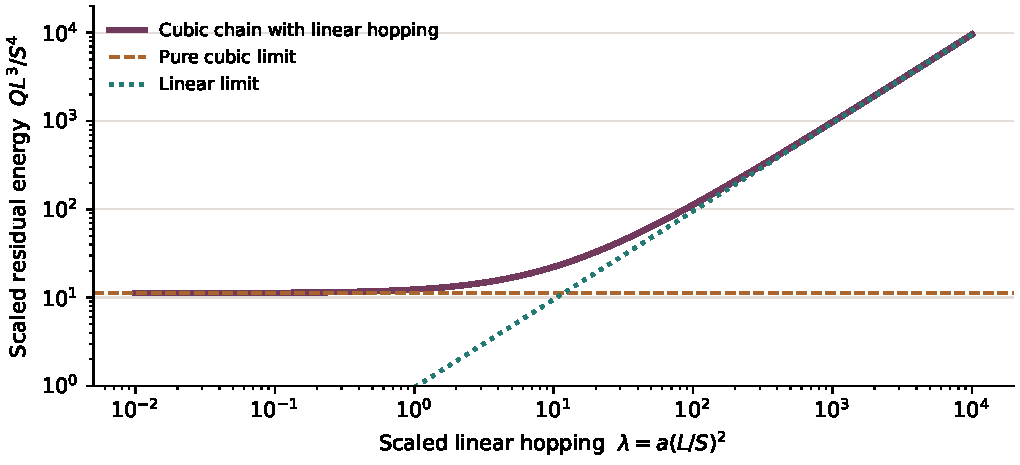
\includegraphics[width=.8\linewidth]{figures/crossover.pdf}
\caption{Cubic-to-linear crossover function $e_3(\lambda)$ from Eq.~\eqref{eq:cross}, with $\lambda=a_L(L/S_L)^{2}$. The vertical scale is $Q_LL^3/S_L^4$. The solid curve is evaluated by quadrature; at $\lambda=1$ it equals $12.34899$, against the pure cubic value $11.20231$. The large-$\lambda$ asymptote is $3\lambda/\pi$.}\label{fig:cross}
\end{figure}
For any fixed $a_L=a>0$, long enough blocks therefore show linear dispersion in the populated range of levels. At $z=3$, comparisons between different lengths probe the crossover when $a$ is of order $(\log L/L)^2$.

\section{What restricted controls leave behind}\label{sec:controls}
This section compares the residual energies left by different classes of operations on the same state and Hamiltonian. It shows that one-body rotations can leave more energy than general unitaries, and that conserving particle number can change the power of $L$.

\subsection{One-body rotations versus general unitaries}
Mula et al.'s Eq.~(34) pairs single-particle occupations with single-particle energies, which minimises the energy over number-conserving Gaussian unitaries, so it computes $Q_L^{\rm G}$. A charge-conserving many-body unitary can permute configurations independently within each particle-number sector, and the unrestricted minimum \eqref{eq:def} also permutes across sectors.
\begin{theorem}[Cost of one-body control]\label{thm:gauss}
For $f(x)=x^z$ with odd $z$, writing $d=\log L$,
\[
 Q_L^{\rm G}\sim \frac{\Gamma(z+1)\eta(z+1)}{\pi^{z+2}}\frac{d^{z+1}}{L^z}.
\]
The ratio $Q_L^{\rm G}/Q_L$ tends to one for $z=1$, has a limit larger than one for every odd $z>1$, and tends to $2.14815$ for $z=3$ and $11.55617$ for $z=5$.
\end{theorem}
\begin{proof}
Let $a_j$ be the sorted absolute one-body energies and $x_j$ the sorted single-particle entanglement energies $|\log((1-\nu_j)/\nu_j)|$, where $\nu_j$ are the block correlation eigenvalues. Staggering the sites reverses the sign of the hopping and exchanges the occupied and empty spectral projectors, so both one-particle spectra have particle--hole pairing, including any zero modes. The one-body trace rearrangement gives $Q_L^{\rm G}=\sum_j a_j/(1+e^{x_j})$.

Appendix~\ref{app:modular} proves $d^{-1}\sum_j\delta_{x_j}\to \dd x/\pi^2$ vaguely on $[0,\infty)$, so $x_j\to\pi^2 y$ whenever $j/d\to y>0$. From the sine spectrum and finite-rank interlacing, $(L/d)^z a_j\to(\pi y)^z$ on the same scale. These quantile limits are uniform on compact subintervals of $y>0$, and
\[
 \int_0^\infty\frac{(\pi y)^z}{1+e^{\pi^2 y}}\dd y
   =\frac{\Gamma(z+1)\eta(z+1)}{\pi^{z+2}} .
\]
For the tails, let $g(t)=\log(1+e^{-t})$. Appendix~\ref{app:modular} bounds $d^{-1}\sum_j g(qx_j)$ for each fixed $q>0$, whence $j/d\le C_qe^{qx_j}$. With $a_j\le C_z(1+j)^z/L^z$ this bounds the normalised sum over $x_j>T$ by $C d^{-1}\sum_{x_j>T}e^{-(1-qz)x_j}=O(e^{-T/2})$, using $q=1/(4z)$ and the bound at $q=1/4$. The part $j<\delta d$ costs $O(\delta^{z+1})+o(1)$.

For strictness, among occupation functions with entropy $\int h(f(y))\dd y=1/6$ ($h$ the binary entropy), the unique minimiser of $\int (\pi y)^z f(y)\dd y$ is the Fermi function $[1+e^{b(\pi y)^z}]^{-1}$ at the entropy-matched $b$. Integrating the nonnegative relative entropy between the two Bernoulli laws proves uniqueness and gives the minimum $D_z/6^{z+1}$ from \eqref{eq:pressure}. The Gaussian occupation $[1+e^{\pi^2 y}]^{-1}$ has entropy $1/6$ and coincides with this minimiser only at $z=1$.
\end{proof}
The ratio concerns residual energies. Their difference, the extra work available to unrestricted controls, tends to zero in absolute terms. At $z=1$ Theorem~\ref{thm:gauss} shows that Mula et al.'s one-body quantity and the many-body bound energy have the same leading law, so their Eq.~(42) holds under either reading. If $R_z=\lim_{L\to\infty}Q_L^{\rm G}/Q_L$, Stirling's formula and $A_z\to\log 2/\pi$ give $R_z^{1/z}/z\to 6\log 2/(e\pi^2)$ as odd $z\to\infty$, each limit $L\to\infty$ being taken at fixed range first. Onuma-Kalu and Mann \cite{onuma} had shown in general that Gaussian operations can fall short of the unrestricted optimum in fermion systems; here the shortfall in residual energy is quantified across a family of chains with a common ground state.

\begin{corollary}[Exact charge conservation]\label{cor:charge}
For $f(x)=x^z$ with odd $z$ (Corollary~\ref{cor:odd}), $Q_L^{\rm ch}/Q_L\to1$, and the same holds for unitaries that preserve only fermion parity. In particular the penalty of Theorem~\ref{thm:gauss} persists when both classes of control conserve charge.
\end{corollary}
Appendix~\ref{app:charge} proves this by counting enough low-energy states at each typical particle number. It parallels the charge-resolved description of entanglement \cite{goldstein}: when particles and holes are equally cheap, every typical charge sector has the full density of low-lying levels.

\subsection{A single chain with three different work-extraction limits}
This subsection shows that particle-number conservation can change the leading power of $L$, even for a Hamiltonian of hopping range three. Let $a=3/2$, $f(x)=x(x-a)^2$, and $H_{2L}=\dd\Gamma(f(T_{2L}))$ with the same physical cut. This $f$ is sign-preserving: $a$ is rational and not $\pm1$. Its ground state is the hopping ground state. In the bulk, removing a particle from just inside the Fermi sea costs energy linear in momentum, while adding one near the second, quadratic zero at $2\cos k=a$ is much cheaper (Fig.~\ref{fig:disp}). This asymmetry between particles and holes separates the three control classes.
\begin{figure}[htbp]\centering
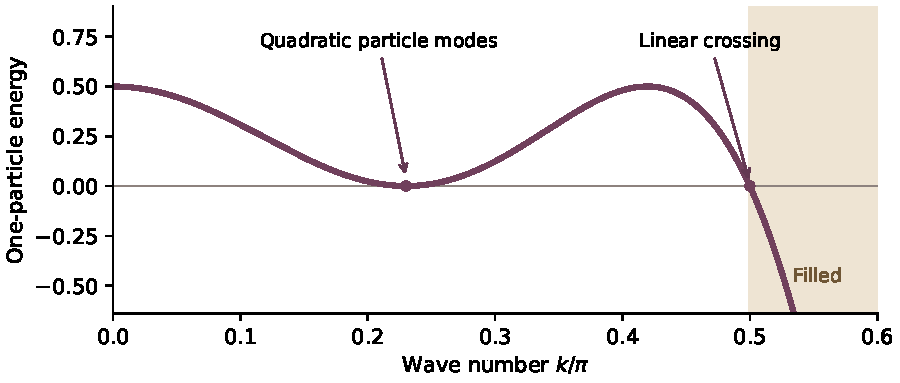
\includegraphics[width=.75\linewidth]{figures/dispersion.pdf}
\caption{One-particle energies $f(2\cos k)$ near their two zeros for $f(x)=x(x-3/2)^2$. The shaded part lies inside the filled Fermi sea, which extends to $k=\pi$. The quadratic minimum lies in the empty part of the band.}\label{fig:disp}
\end{figure}
\begin{theorem}[Three control classes]\label{thm:three}
Put $d=\log L$, $\kappa=a(4-a^2)$, and $A=2\Gamma(3/2)\eta(3/2)/(\pi\sqrt{\kappa})$. For the same block state and the same block Hamiltonian,
\begin{align}
 Q_L &\sim \frac{4}{27A^2}\frac{S_L^3}{L^2},\qquad
 Q_L^{\rm ch} \sim \frac{a^2}{4\pi}\frac{d}{L},\qquad
 Q_L^{\rm G} \sim \frac{a^2}{24\pi}\frac{d^2}{L}.
 \label{eq:three}
\end{align}
The first leading value is also reached by parity-preserving many-body unitaries.
\end{theorem}
\begin{proof}
\emph{Unrestricted control.} This is Theorem~\ref{thm:general} with $m=2$ and the single quadratic zero $a$, for which $c_a=a$ and $\kappa_a=\kappa$; then $D(2,A)=4/(27A^2)$. To reach the same value in either parity sector, reserve one cheapest positive mode, of cost $O(L^{-2})$. Erase its occupation in the full count and choose it to give the required parity. At most two configurations coalesce and the excitation rises by at most $O(L^{-2})$, so the log count at speed $S_L$ is unchanged. The sector rank bound follows by applying the full bound at twice the within-sector rank, and since the probability rank in a sector is at most the full rank, the tail argument still applies.

\emph{Signed one-body levels.} The block matrix differs from $f(T_L)$ by rank at most two. Its number of negative modes $n_*$ is $L/2+O(1)$ and it has $O(1)$ zero modes. Denote the increasing hole and particle costs by $w_j^-$ and $w_j^+$. At $k=\pi/2$ the speed is $v_*=2a^2$, since $f'(0)=a^2$ and $|\dd(2\cos k)/\dd k|=2$ there. Counting the grid $k=\pi j/(L+1)$ up to an $O(1)$ interlacing shift gives, uniformly for $j\le C\log L$,
\[
 w_j^-=\frac{\pi v_*}{L}[j+O(1)]+O(j^2/L^2).
\]
The global bounds are $w_j^-\le C'(j+1)/L$ and $w_j^+\le C'[(j+1)/L]^2$; the positive bound follows by counting modes on both sides of the quadratic zero, and away from it the bounded bandwidth suffices after enlarging $C'$.

\emph{The unavoidable hole cost.} The charge $n$ of a sampled block eigenstate has a distribution symmetric about $L/2$, and by Appendix~\ref{app:modular}
\[
 \frac{\operatorname{Var}n}{d}\to
 \frac{1}{\pi^2}\int_0^\infty \frac{e^x}{(1+e^x)^2}\dd x=\frac{1}{2\pi^2}.
\]
The integrable tail follows from the exponential estimate in the proof of Theorem~\ref{thm:gauss}. Write $k=(n_*-n)_+$ and $c_*=n_*-L/2=O(1)$. Symmetry of $n-L/2$ gives $\E k^2=\E[(L/2+c_*-n)_+^2]=\tfrac12\operatorname{Var}n+O(|c_*|\,\E|n-L/2|+c_*^2)=\tfrac12\operatorname{Var}n+O(\sqrt d+1)$. Any state in sector $n$ costs at least $\sum_{j\le k}w_j^-$, which on $k\le Cd$ equals $\pi v_* k^2/(2L)+O((1+k)/L+k^3/L^2)$. Choose $C$ so large that $\Prob(|n-n_*|>Cd\text{ or }\log R>Cd)=o(L^{-4})$, which Bernstein's inequality for $n$ and the information bound in the proof of Theorem~\ref{thm:general} allow. The total spectral width is $O(L)$, so the complementary event is negligible. Thus the mean compulsory hole cost is asymptotic to $\pi v_*\E k^2/(2L)\sim a^2 d/(4\pi L)$, a lower bound for $Q_L^{\rm ch}$.

\emph{Attaining this cost with number conservation.} For typical $n$ let $j_+=(n-n_*)_+$ and fill the cheapest $j_+$ positive levels. Take $k+H$ holes from the cheapest negative levels, and fill $H$ further particles in any $H$ distinct modes among the next $\lfloor L^{1/3}\rfloor$ cheap positive levels. Here $H$ is a fixed integer larger than $3(C+2)$. Each such configuration has charge $n$, and their number eventually exceeds $L^C$, which is larger than the required within-sector rank. The excess over the compulsory cost is at most
\[
 O_H((1+k)/L)+O((1+j_+)^3/L^2)+O_H(L^{-4/3}).
\]
Since $\E k=O(\sqrt d)$ and $j_+\le Cd$ on the typical event, the mean excess is $o(d/L)$; the spectral width controls the complementary event. This proves the second limit.

\emph{One-body control.} In the signed one-body rearrangement the $j$th hole costs $w_j^-$, and for $j/d\to y>0$ its occupation deficit tends to $[1+e^{2\pi^2 y}]^{-1}$; the factor two arises because each half of the signed entanglement spectrum contains half the levels counted in Appendix~\ref{app:modular}. The shift $n_*-L/2=O(1)$ does not affect this limit. The global one-body bounds and the exponential tail of Theorem~\ref{thm:gauss} justify the Riemann sum. The positive branch contributes only $O(d^3/L^2)$, and the holes give
\[
 \int_0^\infty\frac{\pi v_* y}{1+e^{2\pi^2 y}}\dd y=\frac{v_*}{48\pi}=\frac{a^2}{24\pi}.
\]
This proves the last formula.
\end{proof}

The mechanism is simple. A typical block has a particle number that fluctuates by order $\sqrt{\log L}$. A charge-conserving unitary must leave a corresponding number of holes in the steep, linear branch below the Fermi level, while an unrestricted unitary can put the same probabilities on cheap particle excitations near the quadratic zero. A one-body rotation must in addition respect the ordering of individual occupations. Symmetry-constrained work extraction has been characterised for many copies \cite{mitsu}; Eq.~\eqref{eq:three} gives the single-block costs in physical energy units.

\paragraph{General Gaussian control.} Allowing quadratic operations that create or annihilate pairs gives a fourth entry (Table~\ref{tab:control}). A real orthogonal rotation of the Majorana operators pairs the singular values $|\tanh(x_j/2)|$ of the covariance with the one-body costs $|\varepsilon_j|$; the canonical two-by-two skew blocks and the trace singular-value inequality give the optimum $\sum_j |\varepsilon|_{(j)}/(1+e^{x_j})$ over all orthogonal rotations. A parity-preserving Gaussian rotation has determinant $+1$; if a change of orientation is needed, reversing one axis of the cheapest physical mode costs at most its gap, $O(L^{-2})$. At unsigned rank $j/d\to y>0$ the quadratic levels dominate, with $L^2 |\varepsilon|_{(j)}/d^2\to\kappa(\pi y/2)^2$. Integrating against $(1+e^{\pi^2 y})^{-1}$, with the same tail estimate, gives $Q_L^{\rm pair}\sim\kappa\Gamma(3)\eta(3)d^3/(4\pi^4L^2)$, whose limiting ratio to $Q_L$ is $1.25734\ldots$ at $a=3/2$.

\begin{table}[htbp]\centering\small
\caption{Leading orders of the residual energy in the range-three chain $f(x)=x(x-3/2)^2$. Every entry refers to the same block state and the same block Hamiltonian; $d=\log L$. Number conservation restricts the many-body configurations, and Gaussianity restricts the allowed rotations.}\label{tab:control}
\begin{tabular}{lcc}
\toprule
Allowed block control & Number may change in pairs & Number conserved exactly\\
\midrule
Many-body unitary & $d^3/L^2$ & $d/L$\\
Fermionic Gaussian unitary & $d^3/L^2$ & $d^2/L$\\
\bottomrule
\end{tabular}
\end{table}

\begin{corollary}[Unequal orders of particle and hole dispersion]\label{cor:pq}
Take $f(x)=x^p(x-a)^q$ with $a=3/2$, odd $p\ge1$ and even $q>p$, fixed as $L\to\infty$. Put $V=a^q(2\pi)^p$, $\kappa_q=a^p(4-a^2)^{q/2}$ and $A=2\Gamma(1+1/q)\eta(1+1/q)/(\pi\kappa_q^{1/q})$. If $Z$ is a standard normal variable and $Z_+=\max(Z,0)$, then
\begin{align*}
 Q_L&\sim \frac{q^q}{(q+1)^{q+1}A^q}\frac{S_L^{q+1}}{L^q},\\
 Q_L^{\rm ch}&\sim
 \frac{V\,\E[Z_+^{p+1}]}{(p+1)(2\pi^2)^{(p+1)/2}}
 \frac{(\log L)^{(p+1)/2}}{L^p},\\
 Q_L^{\rm G}&\sim\frac{V\,\Gamma(p+1)\eta(p+1)}{(2\pi^2)^{p+1}}
                    \frac{(\log L)^{p+1}}{L^p}.
\end{align*}
\end{corollary}
\begin{proof}
The first limit is Theorem~\ref{thm:general} with $m=q$. The range is $p+q$ and the ground projector is unchanged. The hole costs obey $w_j^-\sim V(j/L)^p$ for $j\to\infty$, $j/L\to0$, uniformly up to the bounded interlacing shift, and the global upper bounds grow as $[(1+j)/L]^q$ and $[(1+j)/L]^p$ on the positive and negative sides.

The charge is a sum of independent Bernoulli variables whose variance grows as $(\log L)/(2\pi^2)$. The Lindeberg condition holds, and Bernstein tails give convergence of all fixed moments after standardisation. The compulsory $k$ cheapest holes thus have expected cost asymptotic to $V\E[k^{p+1}]/[(p+1)L^p]$, with the displayed Gaussian positive-part moment. For an upper bound reserve $\lfloor L^\theta\rfloor$ positive modes, where $0<\theta<1-p/q$. On $R\le L^C$, a fixed number of reserve particles greater than $(C+1)/\theta$ encodes all ranks as in Theorem~\ref{thm:three}. These particles cost $O(L^{-q(1-\theta)})=o(L^{-p})$, the extra fixed number of holes costs $O((k+1)^p/L^p)$, lower order on average, and typical charge surpluses $O(\log L)$ cost $O((1+\log L)^{q+1}/L^q)$. Choosing $C$ so that the discarded event has probability $o(L^{-p-2})$ proves the second equivalence. For the Gaussian calculation the same signed-level measure gives the coefficient $V\int_0^\infty y^p/(1+e^{2\pi^2 y})\dd y$, and the positive side contributes $O((\log L)^{q+1}/L^q)$, which proves the last equivalence.
\end{proof}

\section{Finite sizes and numerical checks}\label{sec:numerics}
This section reports exact finite-size computations. They test the normalisations and implementations, and they show how quickly, or slowly, the limits of the previous sections are approached. The proofs, not these numbers, carry the limiting statements.

\paragraph{Small chains.} For the odd-power chains, the scripts order all $2^L$ many-body levels through $L=16$. For $L\le6$ they also build the full Slater wavefunction, trace out the complement and diagonalise a spin-basis form of the block Hamiltonian. At $L=6$, $z=1$, the unrestricted value is $Q_L=0.08991246721$ against the one-body value $Q_L^{\rm G}=0.08991382360$. At $L=16$ the same state gives $Q_L=0.05471183245$ for $z=1$ and $0.00787043836$ for $z=3$. For the range-three chain of Theorem~\ref{thm:three}, direct sorting at $L=16$ gives $Q_L=0.00583175688$, $Q_L^{\rm ch}=0.13778687261$ and $Q_L^{\rm G}=0.13822851263$. An interval-arithmetic certificate at $L=5$, $z=1$ shows that $Q_L<Q_L^{\rm G}$ strictly already there: two cheap single-particle flips are $34.84$ times more probable than one expensive flip, yet cost $2-\sqrt3$ more energy, so the one-body ordering is not the many-body optimum.

\paragraph{Ising chain and continuum model.} Table~\ref{tab:checks} gives two independent checks. The spin-basis Ising calculation extends to $2L=16$ spins and agrees with the Majorana calculation to within $2\times10^{-14}$ in residual energy (the script's tolerance is $2\times10^{-13}$). Larger blocks use cross-cut singular values and the 16,384 most probable states and cheapest levels; at $L=2048$ the estimated truncation allowance on $LQ/S^2$ is $2.5\times10^{-8}$, and the calculation is in floating point. In the continuum test the character multiplicities are integers, ranks are matched within degenerate groups, and the Gibbs weights are summed; truncating the entanglement spectrum at $13{,}000$ levels omits less than $3.8\times10^{-19}$ in dimensionless energy at $u=0.016$, by the tilted tail estimate in the code.

\begin{table}[htbp]\centering\small
\caption{Two checks of the conformal law. Left: the critical open Ising chain with its free termination after the cut; the limit is Corollary~\ref{cor:ising}. Right: the free/free and free/fixed Ising annulus spectra of Theorem~\ref{thm:boundary}, with $\mathcal Q=LQ/(\pi v)$ and $K=\pi^2/12$; the limit is the boundary shift $\tfrac12\log2$.}\label{tab:checks}
\begin{tabular}{rr@{\hspace{1cm}}rr}
\toprule
$L$ (spins)& $LQ/S^2$ & $u$ & $2\sqrt{K\mathcal Q}-S$\\
\midrule
8&2.44154&0.200&0.340950\\
32&2.30860&0.100&0.343115\\
128&2.20015&0.025&0.345577\\
2,048&2.07432&0.016&0.345925\\
\midrule
Limit&$6/\pi=1.90986\ldots$&Limit&$\tfrac12\log 2=0.346574\ldots$\\
\bottomrule
\end{tabular}
\end{table}

\paragraph{How fast the limits are reached.} Table~\ref{tab:converge} uses truncated rank matching: the $65{,}536$ most probable Schmidt states against the $65{,}536$ cheapest levels, with estimated omitted probability below $3\times10^{-14}$ at every size (floating point); all chain lengths $2L$ are even. For the range-three chain it also gives a lower bound on $Q_L^{\rm ch}$ that holds at every $L$ and is evaluated exactly up to floating-point rounding: the expected cost of the holes and particles that the block's particle number forces, the quantity whose limit is the hole cost in the proof of Theorem~\ref{thm:three}. Two different behaviours appear. The separation between unrestricted and charge-conserving control in the range-three chain is visible at once and grows with $L$: the lower bound on $Q_L^{\rm ch}$ exceeds $Q_L$ by a factor of about 20 at $L=16$ and about 1,360 at $L=4096$. The odd-$z$ constants converge only logarithmically: for $z=3$ at $L=4096$, $L^3Q_L/S_L^4=36.3$ against the limit $11.20$, and $Q_L^{\rm G}/Q_L=1.096$ against $2.148$. These limits are correct, but at accessible sizes the one-body penalty for $z=3$ is a few per cent, not a factor of two. Likewise the third separation in Table~\ref{tab:control}, between $Q_L^{\rm ch}$ and $Q_L^{\rm G}$, is a factor $(\log L)/6$ in the limit and is not resolved at these sizes.

\begin{table}[htbp]\centering\small
\caption{Finite-size values against the limits proved above. Columns 3--4: the cubic chain $f(x)=x^3$ (Corollary~\ref{cor:odd}, Theorem~\ref{thm:gauss}). Columns 5--7: the range-three chain $f(x)=x(x-3/2)^2$ (Theorem~\ref{thm:three}); ``floor'' is the lower bound on $Q_L^{\rm ch}$ described in the text, and $d=\log L$.}\label{tab:converge}
\begin{tabular}{rrrrrrr}
\toprule
$L$ & $S_L$ & $L^3Q_L/S_L^4$ & $Q_L^{\rm G}/Q_L$ & $L^2Q_L/S_L^3$ & floor$/Q_L$ & $LQ_L^{\rm G}/d^2$\\
\midrule
16 & 0.8468 & 62.69 & 1.0003 & 2.458 & 19.8 & 0.288\\
64 & 1.0917 & 54.34 & 1.0076 & 2.243 & 49.5 & 0.171\\
256 & 1.3263 & 46.56 & 1.0286 & 1.930 & 154 & 0.127\\
1024 & 1.5582 & 40.69 & 1.0596 & 2.079 & 414 & 0.104\\
4096 & 1.7895 & 36.34 & 1.0959 & 1.909 & 1358 & 0.0901\\
\midrule
Limit & $\infty$ & 11.202 & 2.148 & 2.087 & $\infty$ & 0.0298\\
\bottomrule
\end{tabular}
\end{table}

\section{Discussion}\label{sec:discussion}
This section summarises what has been settled, what the results mean physically, and what remains open.

\begin{table}[htbp]\centering\small
\caption{Status of the three forms of the conjecture of Mula et al.\ \cite{mula} after this paper.}\label{tab:status}
\begin{tabular}{>{\raggedright}p{.3\linewidth}>{\raggedright}p{.3\linewidth}p{.3\linewidth}}
\toprule
Form & Status & Where\\
\midrule
(A) $Q_L\propto S_L^2/L$ for all critical ground states & False: one critical ground state carries $S^{m+1}/L^m$ for every $m$ & Theorem~\ref{thm:general}, Corollaries~\ref{cor:odd}, \ref{cor:iff}\\
(B) $Q_L\propto S_L^2/L$ for critical states described by a CFT & Proved for regulated CFT spectra and for the open hopping and critical Ising chains; open for interacting lattice chains & Theorems~\ref{thm:cft}, \ref{thm:boundary}; Corollaries~\ref{cor:iff}, \ref{cor:ising}\\
(C) $NQ_L/S_L^2\to6/\pi$ & True for unit hopping, in both the one-body and many-body readings; in general the slope is $3v/(\pi c)$, e.g.\ $12/\pi$ for the Ising chain with $v=2$. Equal slopes at different $c$ signal different velocities & Corollaries~\ref{cor:iff}, \ref{cor:ising}; Theorem~\ref{thm:gauss}\\
\bottomrule
\end{tabular}
\end{table}

\paragraph{Physical meaning.} The residual energy is set by the low-energy density of levels of the isolated block at the temperature where its thermal entropy equals the entanglement entropy (Remark~\ref{rem:isentropic}). The ground state fixes only that entropy. Whether the familiar $S^2/L$ law results depends on the block Hamiltonian: within the free-fermion family of Section~\ref{sec:lattice} it requires a nonzero Fermi velocity and no other gapless point. This reading is consistent with Mitra and Srivastava's observation \cite{mitra} that the law persists where conformal symmetry is broken by long-range pairing: what matters is the level density at the entanglement temperature, not conformal invariance as such. For experiments that conserve particle number exactly, such as cold atoms in optical lattices, the relevant quantity is $Q_L^{\rm ch}$. Corollary~\ref{cor:charge} and Theorem~\ref{thm:three} give a simple rule: charge conservation costs nothing at leading order when particles and holes are equally cheap, and changes the power of $L$ when one side of the Fermi level is much softer than the other. Table~\ref{tab:converge} shows that this second effect is large already for small blocks.

\paragraph{Limits.} The residual energy is small, of order $(\log L)^2/L$ for ordinary hopping, while the extractable work tends to a constant \cite{mula}. Reaching the minimum requires coherent control of the whole block, with no bound on circuit depth or locality. The theorems describe that ideal. The lattice proofs use one external input, the boundary R\'enyi asymptotics of the open hopping chain (Appendix~\ref{app:renyi}).

\paragraph{Open problems.} (i) A proof of form (B) for an interacting lattice chain, such as the Heisenberg chain, would need control of the number of block levels up to conformal dimensions of order $(\log L)^2$ and of the contribution of rare Schmidt ranks; fixed-level convergence to the CFT does not supply either. (ii) A lattice termination realising different boundary conditions at the cut would test Theorem~\ref{thm:boundary} beyond the continuum model. (iii) The corrections that govern the slow convergence in Table~\ref{tab:converge} are not computed here. (iv) Residual energies under locality- or depth-constrained controls would connect these limits to implementable protocols.

\appendix
\section{R\'enyi data for a finite half-chain}\label{app:renyi}
This appendix supplies the entanglement input used in Theorem~\ref{thm:general}: the R\'enyi entropies of the finite half-chain have the same leading behaviour as those of a block at the end of a semi-infinite chain.

For entropies we may fill the positive subspace instead of the negative one, since the correlation matrix then becomes $1-C$. On $1\le i,j\le L$ the positive Fermi projector restricted from $N=2L$ sites is
\[
 C_{ij}=D_N(i-j)-D_N(i+j),\quad
 D_N(r)=\frac{\sin(\pi r/2)}{2(N+1)\sin[\pi r/(2(N+1))]},\quad D_N(0)=1/2 ,
\]
by summing the first $N/2$ sine modes. For the semi-infinite chain replace $D_N(r)$ by $D_\infty(r)=\sin(\pi r/2)/(\pi r)$. For that block, Fagotti and Calabrese \cite[Eq.~(38)]{fagotti} obtained $S_q=(1+1/q)(\log L)/12+O_q(1)$ for every fixed $q>0$, including $q=1$. They derived it from the asymptotics of Toeplitz-plus-Hankel determinants with Fisher--Hartwig singularities proved by Deift, Its and Krasovsky \cite{dik}, through the standard contour-integral representation of R\'enyi entropies. We take this asymptotic as the one external input of the lattice theorems. We show here that passing to the finite chain changes the required traces by $O_q(1)$, even at block fraction one half.

For $t=r/(N+1)$ the difference $D_N(r)-D_\infty(r)$ equals $(N+1)^{-1}\sin(\pi r/2) f(t)$ with $f(t)=[2\sin(\pi t/2)]^{-1}-(\pi t)^{-1}$, which extends analytically to $|t|<2$. For each $1<\alpha<2$ a degree-$k$ polynomial approximates it to $O(\alpha^{-k})$ uniformly on $[-1,1]$. A polynomial in $i\pm j$ of degree $k$ gives a matrix of rank at most $k+1$, and the sine factor is a sum of two separable exponentials. Therefore $C-C_\infty$ has rank-$4(k+1)$ approximants whose row and column sum errors are $O(\alpha^{-k})$, and its singular values obey $s_j\le C_0e^{-c_0j}$ uniformly in $L$.

For $q\ne1$ let $f_q(x)=\log[x^q+(1-x)^q]$, and let $f_1(x)=-x\log x-(1-x)\log(1-x)$; extend these constantly outside $[0,1]$. Their derivatives on $(0,1)$ are bounded by $C_q[x^{\delta-1}+(1-x)^{\delta-1}]$ for any $0<\delta<\min(q,1)$. A signed rank-one perturbation of trace norm $s$ moves the ordered eigenvalues, by interlacing, over disjoint intervals of total length $s$, and integrating the derivative over these intervals bounds the change of the trace by $C_q s^\delta$, also when intermediate eigenvalues cross an endpoint. Adding the signed eigencomponents of $C-C_\infty$ gives a total change $O(\sum_j s_j^\delta)=O(1)$. The product formula for the eigenvalues of a Gaussian reduced density operator turns these one-body traces into $\log\Tr\rho^q$ and the entropy. This proves the input used in Theorem~\ref{thm:general}, and, for every fixed $q>0$, in Theorem~\ref{thm:gauss}.

\section{Density of the single-particle entanglement levels}\label{app:modular}
This appendix proves that the single-particle entanglement energies $x_j$ have asymptotic density $1/\pi^2$ per unit of $\log L$, the input of Theorems~\ref{thm:gauss} and~\ref{thm:three}.

All block occupations lie strictly between zero and one. Indeed both the occupied and the empty sine-mode submatrices on the first $L$ sites are invertible: $\sin(i k)=\sin k\,U_{i-1}(\cos k)$ with $U_j$ a polynomial of degree $j$, so each determinant is a nonzero weighted Vandermonde determinant. Put $g(y)=\log(1+e^{-y})$, $d=\log L$ and $H_L(q)=d^{-1}\sum_jg(qx_j)$. The Gaussian product identity gives
\[
 d^{-1}\log\Tr\rho_L^q=H_L(q)-qH_L(1),\qquad H_L(1)=-d^{-1}\log\|\rho_L\|_\infty .
\]
For $q>1$, $\|\rho_L\|_\infty^q\le\Tr\rho_L^q\le\|\rho_L\|_\infty^{q-1}$. Using Appendix~\ref{app:renyi} and then letting $q\to\infty$ gives $H_L(1)\to1/12$, and hence $H_L(q)\to 1/(12q)$ for every fixed $q>0$.

Let $\mu_L=d^{-1}\sum_j\delta_{x_j}$. Boundedness of $H_L(q)$ gives locally bounded mass. For each vague limit $\mu$,
$\int g(qx)\dd\mu=1/(12q)$, since above $T$ the integrand is bounded by $C e^{-qT/2}g(qx/2)$. Taking $q=1/x$ gives $\mu[0,x]\le Cx$, so the Laplace transform $M(t)$ of $\mu$ is $O(1/t)$. Expanding $g$ gives $1/(12q)=\sum_n a_nM(nq)$ with $a_n=(-1)^{n+1}/n$. The Dirichlet convolution inverse is $b_n=\sum_{2^k j=n}\mu_{\rm M}(j)/j$, where $\mu_{\rm M}$ is the M\"obius function; this follows from $\sum a_n n^{-s}=(1-2^{-s})\zeta(1+s)$. Since $\sum |b_n|/n\le2\zeta(2)$, both series and their composition converge absolutely, and inversion gives
\[
 M(q)=\sum_n \frac{b_n}{12nq}=\frac{1}{12\eta(2)q}=\frac{1}{\pi^2 q}.
\]
Uniqueness of the Laplace transform identifies every vague limit with $\dd x/\pi^2$. The limit has a positive continuous density, which gives the quantile limits used in the proof of Theorem~\ref{thm:gauss}.

\section{Counting low-energy states at fixed particle number}\label{app:charge}
This appendix proves Corollary~\ref{cor:charge}: for $f(x)=x^z$, where particles and holes are equally cheap, every typical charge sector already contains enough cheap levels.

We use the notation of the proof of Theorem~\ref{thm:general} for $f(x)=x^z$, so that $m=z$, $u=S_L$, $g=u^{m+1}/L^m$, $n_0=\lfloor L/2\rfloor$, and $\sigma(e)$ the right side of \eqref{eq:micro}. Chiral symmetry (staggering the sites reverses the sign of $B_L$) gives a reference ground occupation of charge $n_0$, by filling the negative modes and an appropriate number of zero modes. Interlacing bounds the number of zero modes by $O(1)$.

We first show that the log count, divided by $u$, of levels below $eg$ in any sector $n=n_0+o(u)$ still tends to $\sigma(e)$. The total count gives the upper bound. For the lower bound choose $b$ with $e_b=-F'(b)<e$, and reserve the $m'=\lfloor\theta u\rfloor$ cheapest nonzero particle--hole pairs for a small fixed $\theta>0$. In the unrestricted Gibbs ensemble all occupations are independent. Outside these pairs the mean charge, after restoring the reserve to its ground occupation, is $L/2$, and its variance is $O(u)$, since each Bernoulli variance is at most $2\log(1+e^{-\beta |\varepsilon|})$. The probability that the charge is within $m'/3$ of $L/2$ therefore tends to one, and simultaneously the original energy lies in $(e_b\pm\delta)g$ with probability tending to one. There are at least $\exp\{u[F(b)+b(e_b-\delta)+o(1)]\}$ such configurations.

Erasing the reserve costs at most a factor $2^{2m'}$ in the count. Every distinct outside configuration can then be completed to charge $n$ by at most $m'$ additions or removals in the reserved modes. The extra energy is at most $C\theta^{m+1}g$ for large $L$, since the reserved costs are $O((m'/L)^m)$. Completion preserves distinct outside configurations. Taking $\theta$ and $\delta$ small enough to stay below $eg$, and then letting them tend to zero and $e_b\uparrow e$, proves the count, uniformly on any $o(u)$ window by the sequential form of the argument.

For the $r$th excitation $\mathcal E_{n,r}$ in sector $n$ there is a global bound
\[
 \mathcal E_{n,r}\le C L^{-m}(1+|n-n_0|+\log r)^{m+1}.
\]
Indeed, among the $k$ cheapest nonzero pairs, keeping other occupations at their reference values gives $\binom{2k}{k+n-n_0}$ configurations, at least $2^{c k}$ of them when $|n-n_0|\le k/2$, for an absolute $c>0$. Taking $k$ a large constant multiple of $1+|n-n_0|+\log r$ gives the bound. If the required $k$ exceeds the number of available pairs, the bound follows from the bandwidth, since only $O(1)$ modes are zero.

Under the block state, $n$ is a sum of independent Bernoulli variables with mean $L/2$ and variance at most $u$. Bernstein's inequality gives $\E|n-L/2|^k=O_k(1+u^{k/2})$ for fixed $k>0$. The rank within a charge sector is at most the global probability rank $R$ when ties are broken consistently. With probability tending to one, $|n-n_0|\le u^{2/3}$ and $\log R\le(1+\delta)u$, so the uniform sector count places the energy at this within-sector rank below $eg$ whenever $\sigma(e)>1+\delta$. The global bound, the charge moments and the rank tails justify averaging. Letting $e$ decrease to $D_z$ and $\delta$ to zero gives the unrestricted coefficient also for $Q_L^{\rm ch}$, and the unrestricted minimum gives the opposite inequality. Parity-preserving unitaries include all charge-preserving ones.

\section*{Data and code availability}
The accompanying package contains the manuscript source, all scripts and their outputs. The scripts reproduce every number in Sections~\ref{sec:cft}--\ref{sec:numerics}: complete Fock-space ordering and direct many-body checks for small chains, the interval certificate, the Ising spin and Majorana calculations, the Ising boundary-character counts, the crossover quadrature, the general-dispersion pressure check and the finite-size table. Each check stops with an error if it fails.

\section*{Statement on the use of AI}
AI systems developed and checked the arguments, wrote the code and drafted the text. The work has had internal AI-assisted review and computational checks; it has not had external peer review.

\begin{thebibliography}{20}\small
\bibitem{allahverdyan} A. E. Allahverdyan, R. Balian and Th. M. Nieuwenhuizen (2004). Maximal work extraction from finite quantum systems. \emph{Europhysics Letters}, 67, 565--571. \url{https://doi.org/10.1209/epl/i2004-10101-2}
\bibitem{alba} V. Alba, P. Calabrese and E. Tonni (2018). Entanglement spectrum degeneracy and the Cardy formula in 1+1 dimensional conformal field theories. \emph{Journal of Physics A: Mathematical and Theoretical}, 51, 024001. \url{https://doi.org/10.1088/1751-8121/aa9365}
\bibitem{alicki} R. Alicki and M. Fannes (2013). Entanglement boost for extractable work from ensembles of quantum batteries. \emph{Physical Review E}, 87, 042123. \url{https://doi.org/10.1103/PhysRevE.87.042123}
\bibitem{ingham} K. Bringmann, C. Jennings-Shaffer and K. Mahlburg (2023). On a Tauberian theorem of Ingham and Euler--Maclaurin summation. \emph{The Ramanujan Journal}, 61, 55--86. \url{https://doi.org/10.1007/s11139-020-00377-5}
\bibitem{calabrese} P. Calabrese and A. Lefevre (2008). Entanglement spectrum in one-dimensional systems. \emph{Physical Review A}, 78, 032329. \url{https://doi.org/10.1103/PhysRevA.78.032329}
\bibitem{cardy} J. Cardy (2004, revised 2008). Boundary conformal field theory. arXiv:hep-th/0411189v2. \url{https://arxiv.org/abs/hep-th/0411189}
\bibitem{tonni} J. Cardy and E. Tonni (2016). Entanglement Hamiltonians in two-dimensional conformal field theory. \emph{Journal of Statistical Mechanics: Theory and Experiment}, 2016, 123103. \url{https://doi.org/10.1088/1742-5468/2016/12/123103}
\bibitem{dik} P. Deift, A. Its and I. Krasovsky (2011). Asymptotics of Toeplitz, Hankel, and Toeplitz+Hankel determinants with Fisher--Hartwig singularities. \emph{Annals of Mathematics}, 174, 1243--1299. \url{https://doi.org/10.4007/annals.2011.174.2.12}
\bibitem{fagotti} M. Fagotti and P. Calabrese (2011). Universal parity effects in the entanglement entropy of XX chains with open boundary conditions. \emph{Journal of Statistical Mechanics: Theory and Experiment}, 2011, P01017. \url{https://doi.org/10.1088/1742-5468/2011/01/P01017}
\bibitem{goldstein} M. Goldstein and E. Sela (2018). Symmetry-resolved entanglement in many-body systems. \emph{Physical Review Letters}, 120, 200602. \url{https://doi.org/10.1103/PhysRevLett.120.200602}
\bibitem{hartmann} D. Hartmann, K. Kavanagh and S. Vandoren (2021). Entanglement entropy with Lifshitz fermions. \emph{SciPost Physics}, 11, 031. \url{https://doi.org/10.21468/SciPostPhys.11.2.031}
\bibitem{igloi} F. Igl\'oi and R. Juh\'asz (2008). Exact relationship between the entanglement entropies of XY and quantum Ising chains. \emph{EPL}, 81, 57003. \url{https://doi.org/10.1209/0295-5075/81/57003}
\bibitem{mitra} A. Mitra and S. C. L. Srivastava (2025). Bound energy, entanglement and identifying critical points in 1D long-range Kitaev model. \emph{New Journal of Physics}, 27, 084601. \url{https://doi.org/10.1088/1367-2630/adf2d2}
\bibitem{mitsu} Y. Mitsuhashi, K. Kaneko and T. Sagawa (2022). Characterizing symmetry-protected thermal equilibrium by work extraction. \emph{Physical Review X}, 12, 021013. \url{https://doi.org/10.1103/PhysRevX.12.021013}
\bibitem{mula} B. Mula, E. M. Fern\'andez, J. E. Alvarellos, J. J. Fern\'andez, D. Garc\'ia-Aldea, S. N. Santalla and J. Rodr\'iguez-Laguna (2023). Ergotropy and entanglement in critical spin chains. \emph{Physical Review B}, 107, 075116. \url{https://doi.org/10.1103/PhysRevB.107.075116}
\bibitem{onuma} M. Onuma-Kalu and R. B. Mann (2018). Work extraction using Gaussian operations in noninteracting fermionic systems. \emph{Physical Review E}, 98, 042121. \url{https://doi.org/10.1103/PhysRevE.98.042121}
\end{thebibliography}
\end{document}
